% \iffalse
\documentclass[journal,12pt,twocolumn]{IEEEtran}
\usepackage{cite}
\usepackage{amsmath,amssymb,amsfonts,amsthm}
\usepackage{algorithmic}
\usepackage{graphicx}
\usepackage{textcomp}
\usepackage{xcolor}
\usepackage{txfonts}
\usepackage{listings}
\usepackage{enumitem}
\usepackage{mathtools}
\usepackage{gensymb}
\usepackage{comment}
\usepackage[breaklinks=true]{hyperref}
\usepackage{tkz-euclide}
\usepackage{listings}
\usepackage{gvv}
\def\inputGnumericTable{}
\usepackage[latin1]{inputenc}
\usepackage{color}
\usepackage{array}
\usepackage{longtable}
\usepackage{calc}
\usepackage{multirow}
\usepackage{hhline}
\usepackage{ifthen}
\usepackage{lscape}
\usepackage{caption}

\newtheorem{theorem}{Theorem}[section]
\newtheorem{problem}{Problem}
\newtheorem{proposition}{Proposition}[section]
\newtheorem{lemma}{Lemma}[section]
\newtheorem{corollary}[theorem]{Corollary}
\newtheorem{example}{Example}[section]
\newtheorem{definition}[problem]{Definition}
\newcommand{\BEQA}{\begin{eqnarray}}
\newcommand{\EEQA}{\end{eqnarray}}
\newcommand{\define}{\stackrel{\triangle}{=}}
\theoremstyle{remark}
\newtheorem{rem}{Remark}
\begin{document}

\bibliographystyle{IEEEtran}
\vspace{3cm}

\title{GATE: CE - 30.2023}
\author{EE23BTECH11010 - Venkatesh D Bandawar $^{*}$% <-this % stops a space
}
\maketitle
% \newpage
\bigskip

% \renewcommand{\thefigure}{\theenumi}
% \renewcommand{\thetable}{\theenumi}

\textbf{Question:} In the differential equation $\frac{dy}{dx} + \alpha x y = 0, \alpha$ is a positive constant. If $y = 1.0$ at
$x = 0.0$, and $y = 0.8$ at $x = 1.0$, the value of $\alpha$ is (rounded off to three decimal places).  \hfill(GATE CE 2023)

\solution
\begin{table}[!h] 
\centering
\begin{tabular}{|c|c|c|}
\hline
    Parameter & Description & Value\\
    \hline
    $P(s)$ & Plant Transfer Function & $\frac{0.001}{s\brak{\frac{s}{0.5}+1}\brak{\frac{s}{100}+1}}$\\
    \hline
    $C(s)$ & Lag Compensator  & $\frac{100\brak{\frac{s}{10}+1}}{\frac{s}{0.1}+1}$\\
    \hline
    $T(s)$ & Loop gain  & $P(s) C(s)$ \\
    \hline
    $\omega$ & Angular Frequency & 3rad/s \\
    \hline
\end{tabular}

\caption{Given parameters}
\label{given parameters list.gate.ce.30}
\end{table}

% \begin{align}
%     \frac{dy}{dx} + \alpha x y &= 0\\
%     \int \frac{dy}{y} &= - \int \alpha x dx\\
%     \ln(\abs{y}) &= - \frac{\alpha x^2}{2} + c
% \end{align}
% Substituting $x$ and $y$ values,
% \begin{align}
%     c &= \ln(1) = 0\\
%     \alpha &= -2 \ln(0.8) = 0.446
% \end{align}


let, $t=x$
\begin{align}
    \frac{dy}{dt} + \alpha t y &= 0
\end{align}
Taking fourier transform,
where,
\begin{align}
    \frac{dy}{dt} & \system{\mathcal{F}} j 2\pi f Y(f) \label{fourier transform of dy/dt_ce_30}\\
    a \cdot t \cdot y(t) & \system{\mathcal{F}} a \cdot \frac{j}{2\pi} \frac{d}{df} Y(f)\label{fourier transform of aty_ce_30}
\end{align}
From equation \eqref{fourier transform of dy/dt_ce_30} and \eqref{fourier transform of aty_ce_30}:
\begin{align}
    \frac{4\pi^2 f}{\alpha} Y(f) + \frac{d}{df} Y(f) &= 0\\
    Y(f) &= K e^{-\frac{4\pi^2 f^2}{2\alpha} }
\end{align}

Taking inverse fourier transform, Using gaussian integral,
WKT, 
\begin{align}
     e^{-a\brak{2\pi f}^2} \mathrel{\substack{\mathcal{F}^{-1}\\\longleftrightarrow}} \frac{1}{\sqrt{4\pi a}} e^{-\frac{t^2}{4a}}
\end{align}
From \tabref{given parameters list.gate.ce.30}:
\begin{align}
    y(t) &= K \frac{\alpha}{\sqrt{2\pi}} e^{-\frac{\alpha t^2}{2}}\\
    \frac{y(0)}{y(1)} &= \frac{1}{e^{-\frac{\alpha}{2}}}\\
    \ln\frac{5}{4} &= \frac{\alpha}{2} \\
    \alpha &= 0.446 
\end{align}

\begin{figure}[!h] 
    \centering
    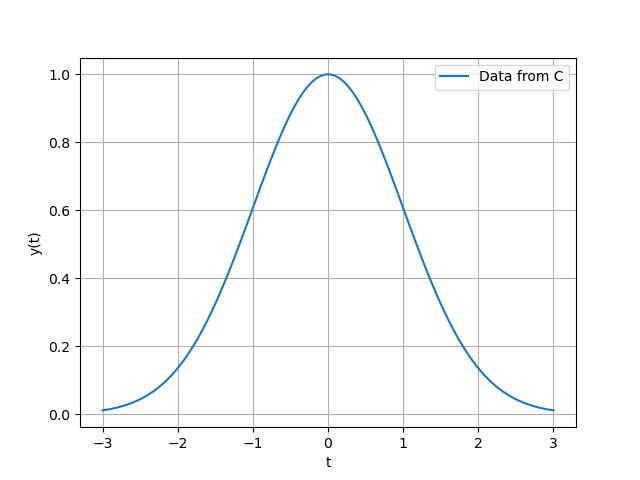
\includegraphics[width=\columnwidth]{figs/graph_of_y(t).png}
    \caption{Graph of y(t)}
    \label{fig:Graph1_gate_CE_30}
    \end{figure}

\end{document}
